\documentclass[10pt]{beamer}

\usetheme{Madrid}
\usecolortheme{default}
\setbeamertemplate{navigation symbols}{}
\setbeamertemplate{footline}[frame number]

\usepackage[utf8]{inputenc}
\usepackage[T1]{fontenc}
\usepackage{lmodern}
\usepackage{amsmath}
\usepackage{amssymb}
\usepackage{graphicx}
\usepackage{booktabs}
\usepackage{listings}
\usepackage{xcolor}

\lstdefinestyle{code}{
  basicstyle=\ttfamily\tiny,
  breaklines=true,
  columns=fullflexible,
  keywordstyle=\bfseries\color{blue!60!black},
  commentstyle=\color{teal},
  language=Python,
}

\title[F2 $\tan(x)$ -- D2]{A User-Centred, From-Scratch Scientific Calculator\\ for the Tangent Function $\tan(x)$}
\subtitle{Deliverable 2: From-Scratch Implementation, Tkinter GUI, VCS, Updated Requirements}
\author{Risat Ahmed \\ \small Student ID: 40294116}
\institute{SOEN 6011 -- Software Engineering Processes, Section CC \\ Concordia University -- Summer 2026}
\date{July 29, 2026}

\begin{document}

\begin{frame}
  \titlepage
\end{frame}

\begin{frame}{Outline}
  \tableofcontents
\end{frame}

\section{From-Scratch Boundary}
\begin{frame}{Problem 5 --- Interpreting ``From Scratch''}
  \textbf{D1 status:} $\sin$/$\cos$ already from scratch (Maclaurin series); only \texttt{PI = math.pi} remained.

  \vspace{0.3cm}
  \textbf{Interpretation adopted (decision D-06):}
  \begin{itemize}
    \item \textbf{Prohibited:} a library call that itself computes a trig/transcendental result (\texttt{math.sin/cos/tan/atan/pi}).
    \item \textbf{Permitted:} ordinary arithmetic (\texttt{+ - * /}), I/O, the Tkinter toolkit.
  \end{itemize}

  \vspace{0.3cm}
  \textbf{Consequence:} Algorithm A (Maclaurin) already satisfies the constraint once \texttt{PI} is independent $\Rightarrow$ \textbf{retained}, reversing D1's forward note toward CORDIC.

  \vspace{0.2cm}
  Verified: \texttt{grep -rn "math\textbackslash." src/} $\to$ no matches outside prose.
\end{frame}

\begin{frame}[fragile]{From-Scratch $\pi$ --- Machin's Identity}
  \[
  \frac{\pi}{4} = 4\arctan\!\left(\tfrac{1}{5}\right) - \arctan\!\left(\tfrac{1}{239}\right)
  \]
  \begin{lstlisting}[style=code]
def _arctan_series(y, tol, n_max):
    term = y; total = y; y2 = y*y; n = 1
    while abs(term) >= tol and n <= n_max:
        term = term * (-y2) * (2*n-1) / (2*n+1)
        total += term; n += 1
    return total

PI = 16*_arctan_series(1/5) - 4*_arctan_series(1/239)
  \end{lstlisting}
  Converges in $\sim$13 terms to $10^{-18}$; matches \texttt{math.pi} to $8.9\times10^{-16}$.
\end{frame}

\section{Numerical Core}
\begin{frame}{Numerical Architecture (D2-P5.2)}
  \begin{columns}
    \begin{column}{0.5\textwidth}
      \texttt{constants.py} -- from-scratch \texttt{PI}

      \texttt{exceptions.py} -- \texttt{NumericalRangeError}, \texttt{DomainError}, \texttt{ConvergenceError}

      \texttt{trig\_series.py} -- \texttt{maclaurin\_sin/cos}
    \end{column}
    \begin{column}{0.5\textwidth}
      \texttt{validation.py} -- parsing + deg/rad

      \texttt{tan\_core.py} -- pure \texttt{tan(x, tolerance, max\_terms)}, no I/O
    \end{column}
  \end{columns}
  \vspace{0.3cm}
  Series functions now \textbf{raise} \texttt{ConvergenceError} on exhaustion instead of D1's silent stop -- closes a REL-01 gap.
  \vspace{0.2cm}
  Core is importable/testable without launching the GUI; both \texttt{cli.py} and \texttt{gui.py} call it as their only numerical dependency.
\end{frame}

\section{Tkinter GUI}
\begin{frame}{Problem 5 --- GUI Wireframe (before code)}
  \begin{itemize}
    \item $x$ entry, label updates with unit ("x in radians"/"x in degrees")
    \item Radians/degrees radio buttons, radians default
    \item Domain hint shown \emph{before} any error can occur
    \item Calculate/Clear buttons + Enter/Esc key bindings
    \item Status text always prefixed "Error"/"OK" -- never colour alone
  \end{itemize}
\end{frame}

\begin{frame}{GUI --- Valid Result}
  \centering
  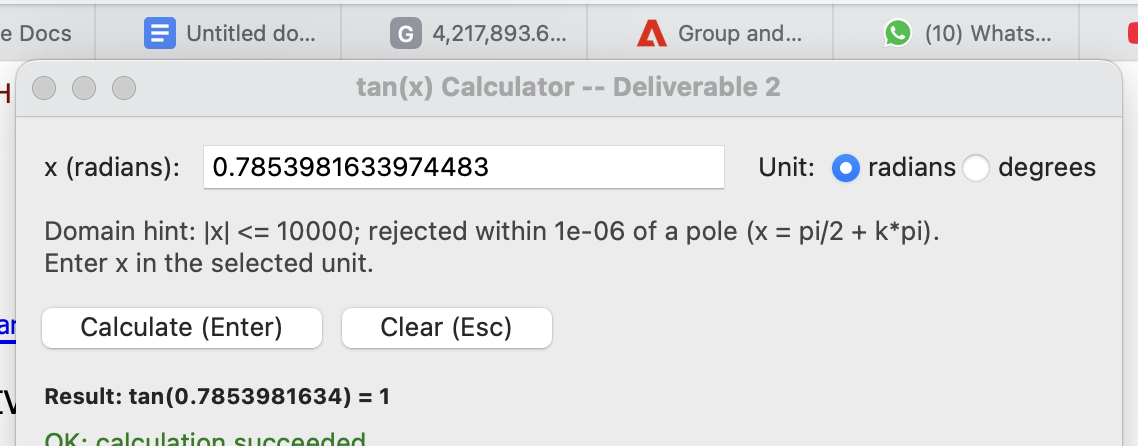
\includegraphics[width=0.78\textwidth]{../../docs/screenshots/d2_gui_valid_pi4.png}
\end{frame}

\begin{frame}{GUI --- Near-Pole Rejection (No Traceback)}
  \centering
  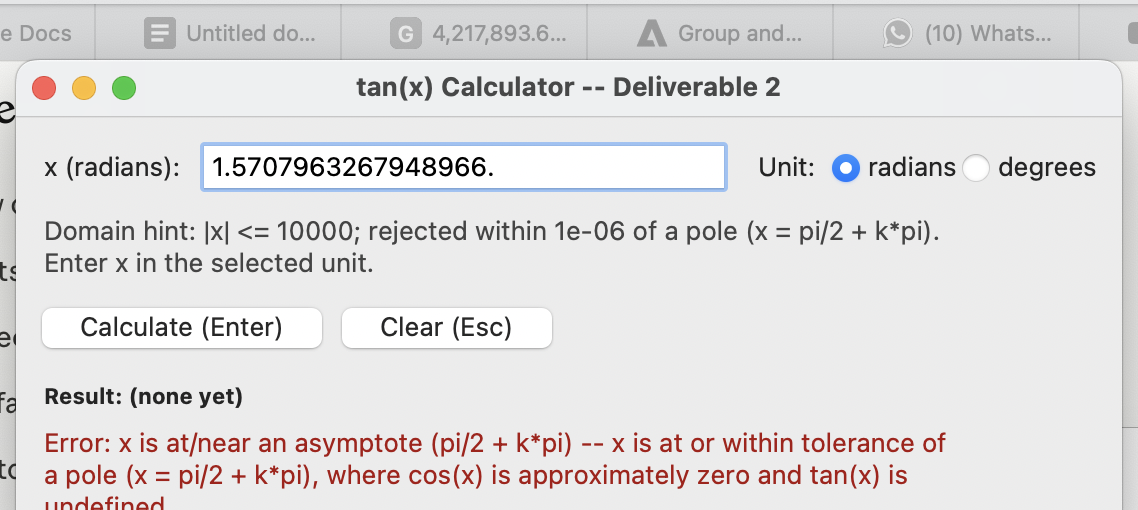
\includegraphics[width=0.78\textwidth]{../../docs/screenshots/d2_gui_near_pole.png}
\end{frame}

\section{Repository \& README}
\begin{frame}{Problem 6 --- Repository \& Commit History}
  \begin{itemize}
    \item D1 submitted as a Moodle zip before Git init -- stated honestly as one baseline commit, not fabricated/backdated history
    \item D2: \textbf{11 cohesive, per-concern commits} (boundary doc $\to$ core $\to$ CLI migration $\to$ wireframe $\to$ GUI $\to$ verification $\to$ README $\to$ requirements $\to$ decision/GAI logs $\to$ report)
    \item \texttt{README.md}: purpose, run commands (\texttt{python3 -m src.cli}/\texttt{src.gui}), usage examples, error/troubleshooting table, honest known-limitations section
  \end{itemize}
\end{frame}

\section{Updated Requirements}
\begin{frame}{Problem 7 --- Baseline v0.2 Changelog}
  \footnotesize
  \begin{table}
    \begin{tabular}{@{}p{1.1cm}p{1.6cm}p{7.2cm}@{}}
      \toprule
      ID & Change & What changed \\
      \midrule
      FR-07 & New & Labelled degrees input mode (D-08) \\
      USE-03 & New & Tkinter GUI, keyboard nav, no colour-only errors \\
      DEP-01 & New & Core shall not call \texttt{math.sin/cos/tan/pi} \\
      ERR-03 & New & 3 named exception types, not bare \texttt{Exception} \\
      ACC-01 & Revised & Bound unchanged; near-pole margin ($3.83\times10^{-10}$) flagged tight, not weakened \\
      \bottomrule
    \end{tabular}
  \end{table}
  13 v0.1 requirements unchanged and still in force. v0.1 retained on disk (C-06).
\end{frame}

\section{Verification}
\begin{frame}{Verification --- 15/15 Cases Pass}
  \begin{table}
    \small
    \begin{tabular}{lll}
      \toprule
      Case & Result & Verdict \\
      \midrule
      $x=\pi/4$ & rel.\ err.\ $1.4\times10^{-15}$ & Pass \\
      $x=1000$ & rel.\ err.\ $5.6\times10^{-13}$ & Pass \\
      $x=\pi/2-10^{-6}$ (near pole) & rel.\ err.\ $3.8\times10^{-10}$ & Pass (tightest) \\
      $x=\pi/2$ (at pole) & \texttt{DomainError} raised & Pass (rejected) \\
      $x=10^{10}$ & \texttt{NumericalRangeError} raised & Pass (rejected) \\
      \bottomrule
    \end{tabular}
  \end{table}
  Reference: independent \texttt{math.tan}, never the algorithm verifying itself. Full matrix: \texttt{docs/verification\_matrix\_d2.md}.
\end{frame}

\begin{frame}{Known Limitations (Honest Disclosure)}
  \begin{itemize}
    \item $|x|\le10^4$ range bound unchanged, still provisional pending professor confirmation
    \item Near-pole relative error ($3.8\times10^{-10}$) is the tightest margin to the $10^{-9}$ ceiling of any passing case
    \item No performance/timing requirement verified (deliberately out of scope)
    \item Formal PyUnit suite is a D3 deliverable; D2 verification is a standalone script
  \end{itemize}
\end{frame}

\section{GAI Prompts}
\begin{frame}{GAI Prompt --- Problem 5 (Core + GUI)}
  \footnotesize
  \textbf{Tool:} Claude Code (Sonnet 5) \quad \textbf{Type:} Generative + architectural
  \begin{description}
    \item[TASK] Freeze the from-scratch boundary; design/implement a pure \texttt{tan(x, tolerance, max\_terms)} core with named exceptions; wireframe then implement a Tkinter GUI; verify against references.
    \item[RESTRICTIONS] No \texttt{math.sin/cos/tan/pi} in the compute path; core importable without the GUI; no unhandled traceback.
    \item[OUTPUT FORMAT] Boundary doc, core modules, wireframe doc, \texttt{gui.py}, verification matrix.
    \item[AUDIENCE] SOEN 6011 grading audience -- evidence-based, traceable to VAL/ACC/ERR/REL requirements.
  \end{description}
\end{frame}

\begin{frame}{GAI Prompt --- Problem 6 \& 7}
  \footnotesize
  \textbf{Problem 6 --- TASK:} cohesive incremental commits by concern; a README a stranger can run the project from. \textbf{RESTRICTIONS:} no secrets/IDE files committed; README claims checked, not assumed.

  \vspace{0.3cm}
  \textbf{Problem 7 --- TASK:} compare every v0.1 requirement against D2 evidence; add/revise with a ``discovered via'' note; freeze v0.2. \textbf{RESTRICTIONS:} keep v0.1 on disk; no silent deletions; no unverifiable requirement wording (e.g.\ ``visually appealing'' rejected, replaced with concrete USE-03).
\end{frame}

\section{References}
\begin{frame}{References}
  \small
  \begin{itemize}
    \item ISO/IEC/IEEE 29148:2018, Requirements Engineering.
    \item J. E. Volder, ``The CORDIC Trigonometric Computing Technique,'' \emph{IRE Trans.\ Electronic Computers}, 1959.
    \item J.-M. Muller et al., \emph{Handbook of Floating-Point Arithmetic}, 2nd ed., 2016.
    \item NIST Digital Library of Mathematical Functions, \url{https://dlmf.nist.gov/}.
  \end{itemize}
\end{frame}

\begin{frame}{Thank You}
  \centering
  \Large Questions?
\end{frame}

\end{document}
